%!TEX root = ../talk.tex

\section{Comparison}\label{sec:numer}

%%%

\frameinlbffalse

{
\usebackgroundtemplate{
\tikz[overlay,remember picture] \node[opacity=0.4, at=(current page.center)] {
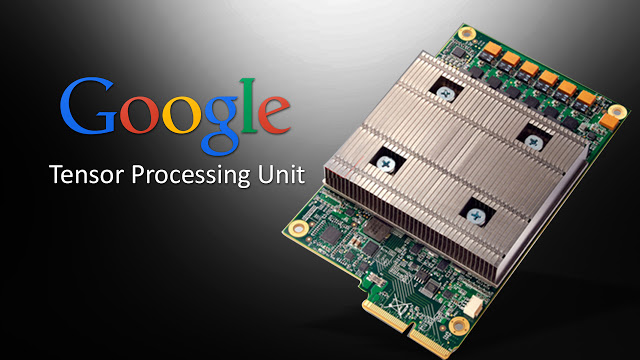
\includegraphics[width=1.15\paperwidth,height=0.68\paperwidth]{figures/tpu.jpg}
};}

\begin{frame}[plain]
\frametitle{\S\ref{sec:numer}. \insertsection}
\listofframes
\end{frame}
\addtocounter{framenumber}{-1} % this page does not count

}

\frameinlbftrue

%%%
\subsection{CPU tests}
%%%

\begin{frame}
	\MyLogo
	\frametitle{CPU Scalability: FCN Synthetic}  

\begin{figure}[htbp] 
	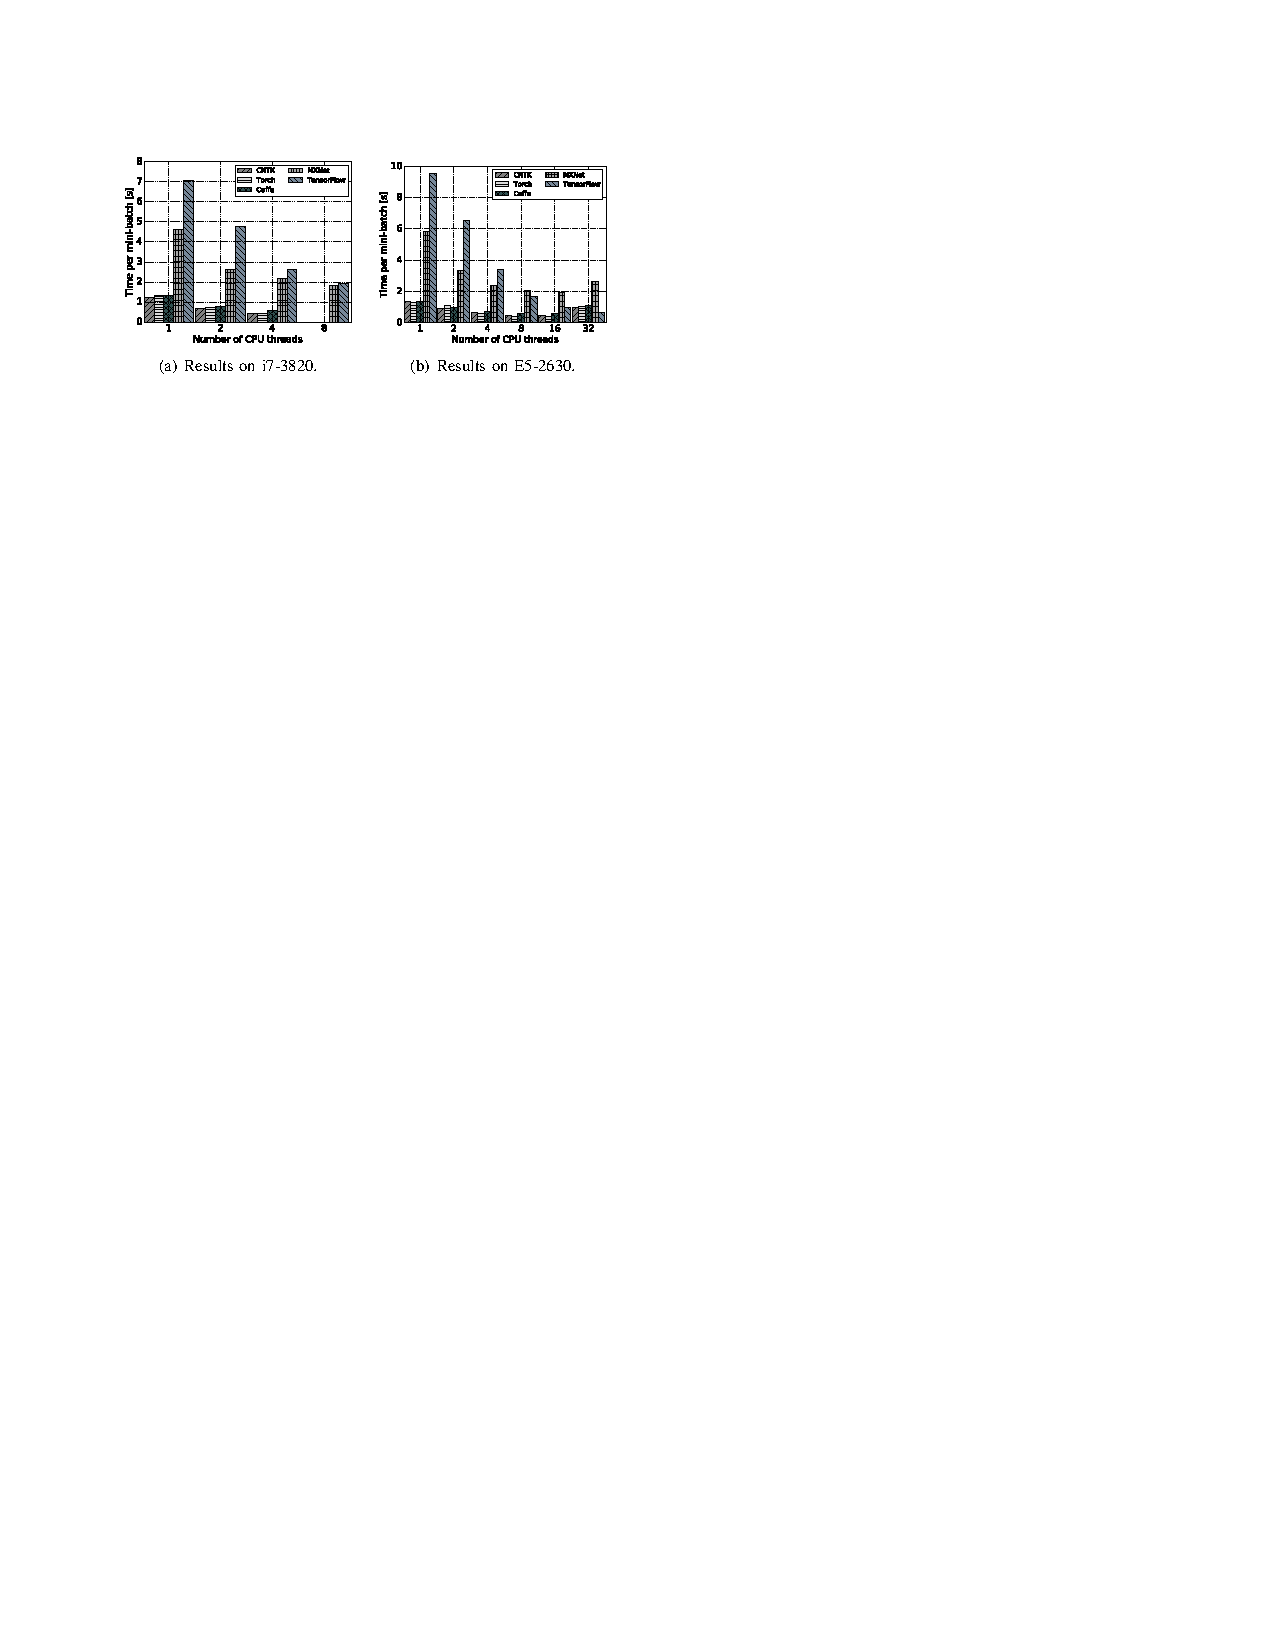
\includegraphics[width=\linewidth]{figures/FCN-S1.pdf} 
	\caption{FCN-S performance on CPU platform with a mini-batch size of 64}
\end{figure}
	
\vskip -10pt
\begin{mdframed}[style=mystyle1]
\begin{itemize}
\item CNTK/Torch/Caffe have similar CPU performance
\item TensorFlow has excellent scalability
\end{itemize}
\end{mdframed}

\end{frame}

%%%

\begin{frame}
	\MyLogo
	\frametitle{CPU Scalability: FCN Real}  
	\begin{figure}[htbp] 
		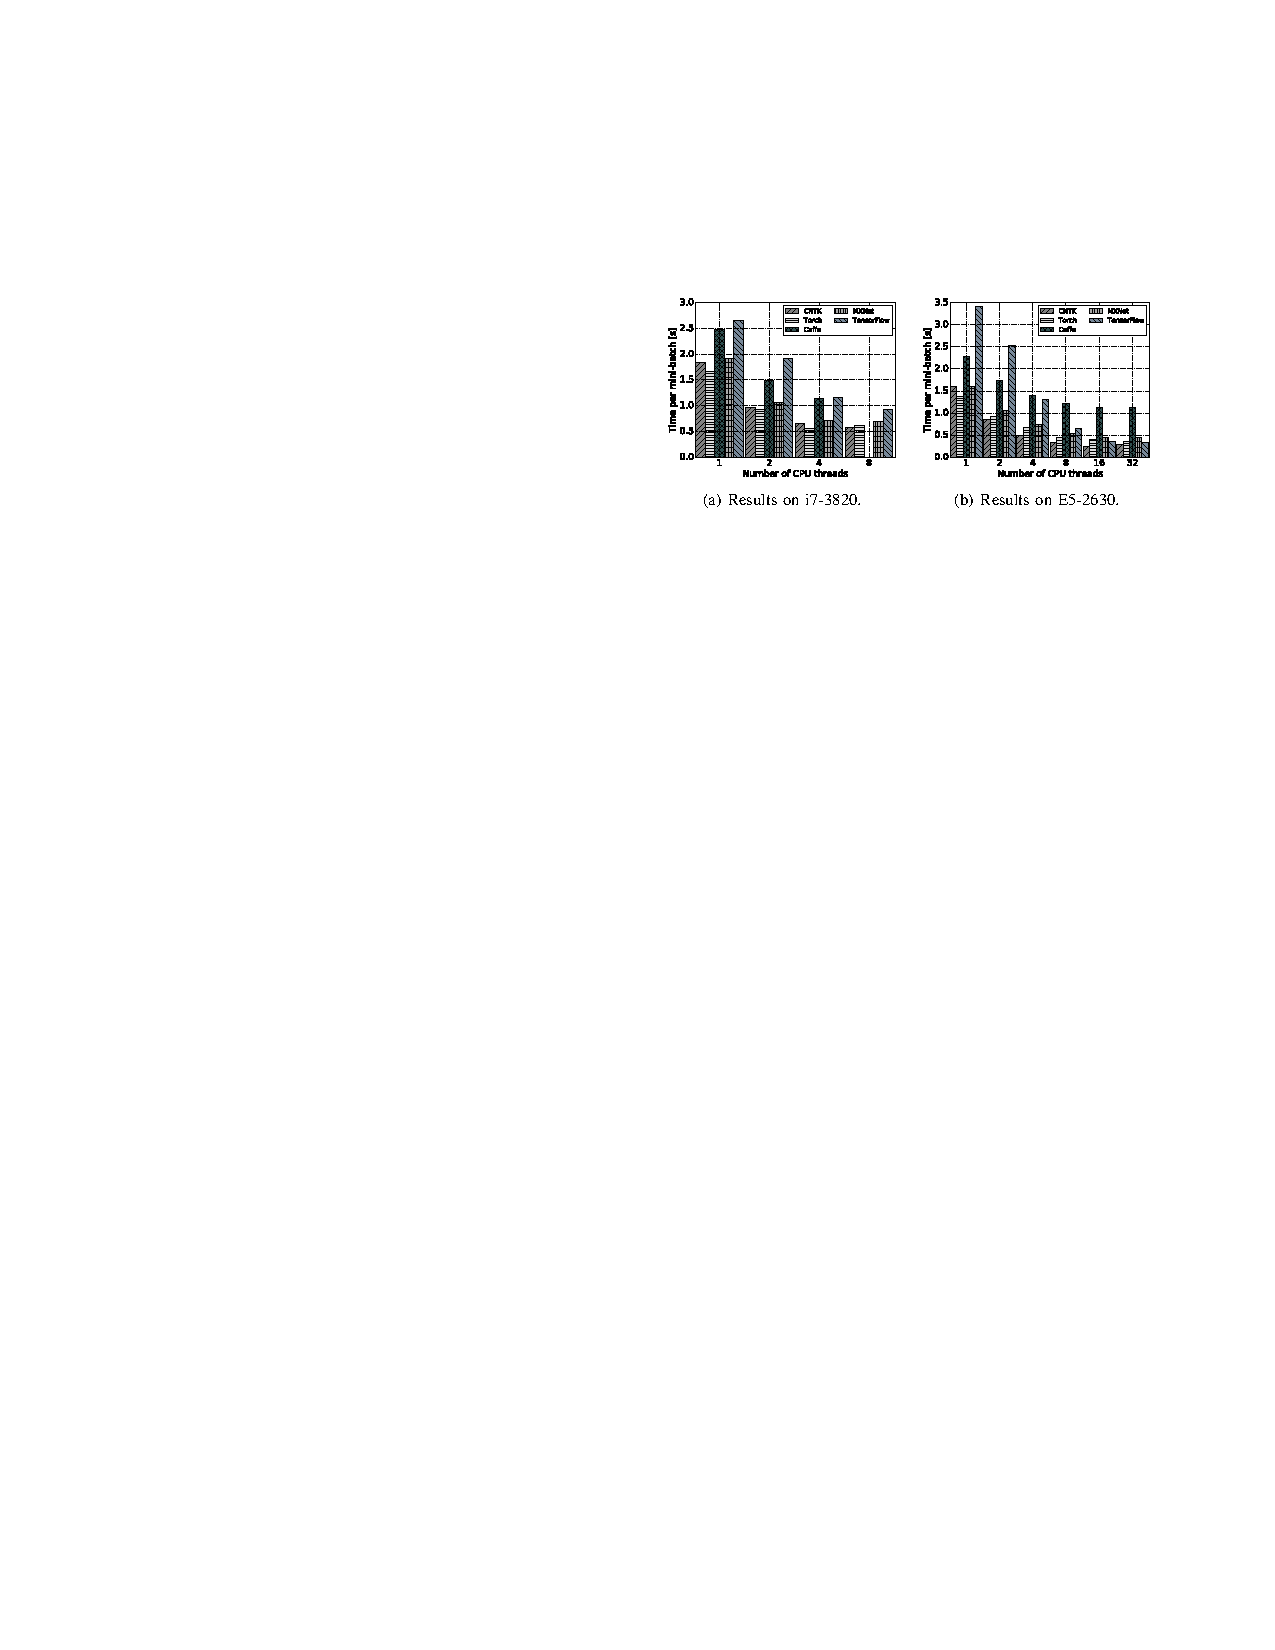
\includegraphics[width=\linewidth]{figures/FCN-R1.pdf} 
		\caption{The FCN-R performance on CPU platform with a mini-batch size of 1024}
	\end{figure}
	
\vskip -10pt
\begin{mdframed}[style=mystyle1]
\begin{itemize}
\item All engines have good CPU performance
\item TensorFlow has good scalability but considerably slower
\end{itemize}
\end{mdframed}

\end{frame}

%%%

\begin{frame}
	\MyLogo
	\frametitle{CPU Scalability: CNN Synthetic}  

	\begin{figure}[htbp] 
		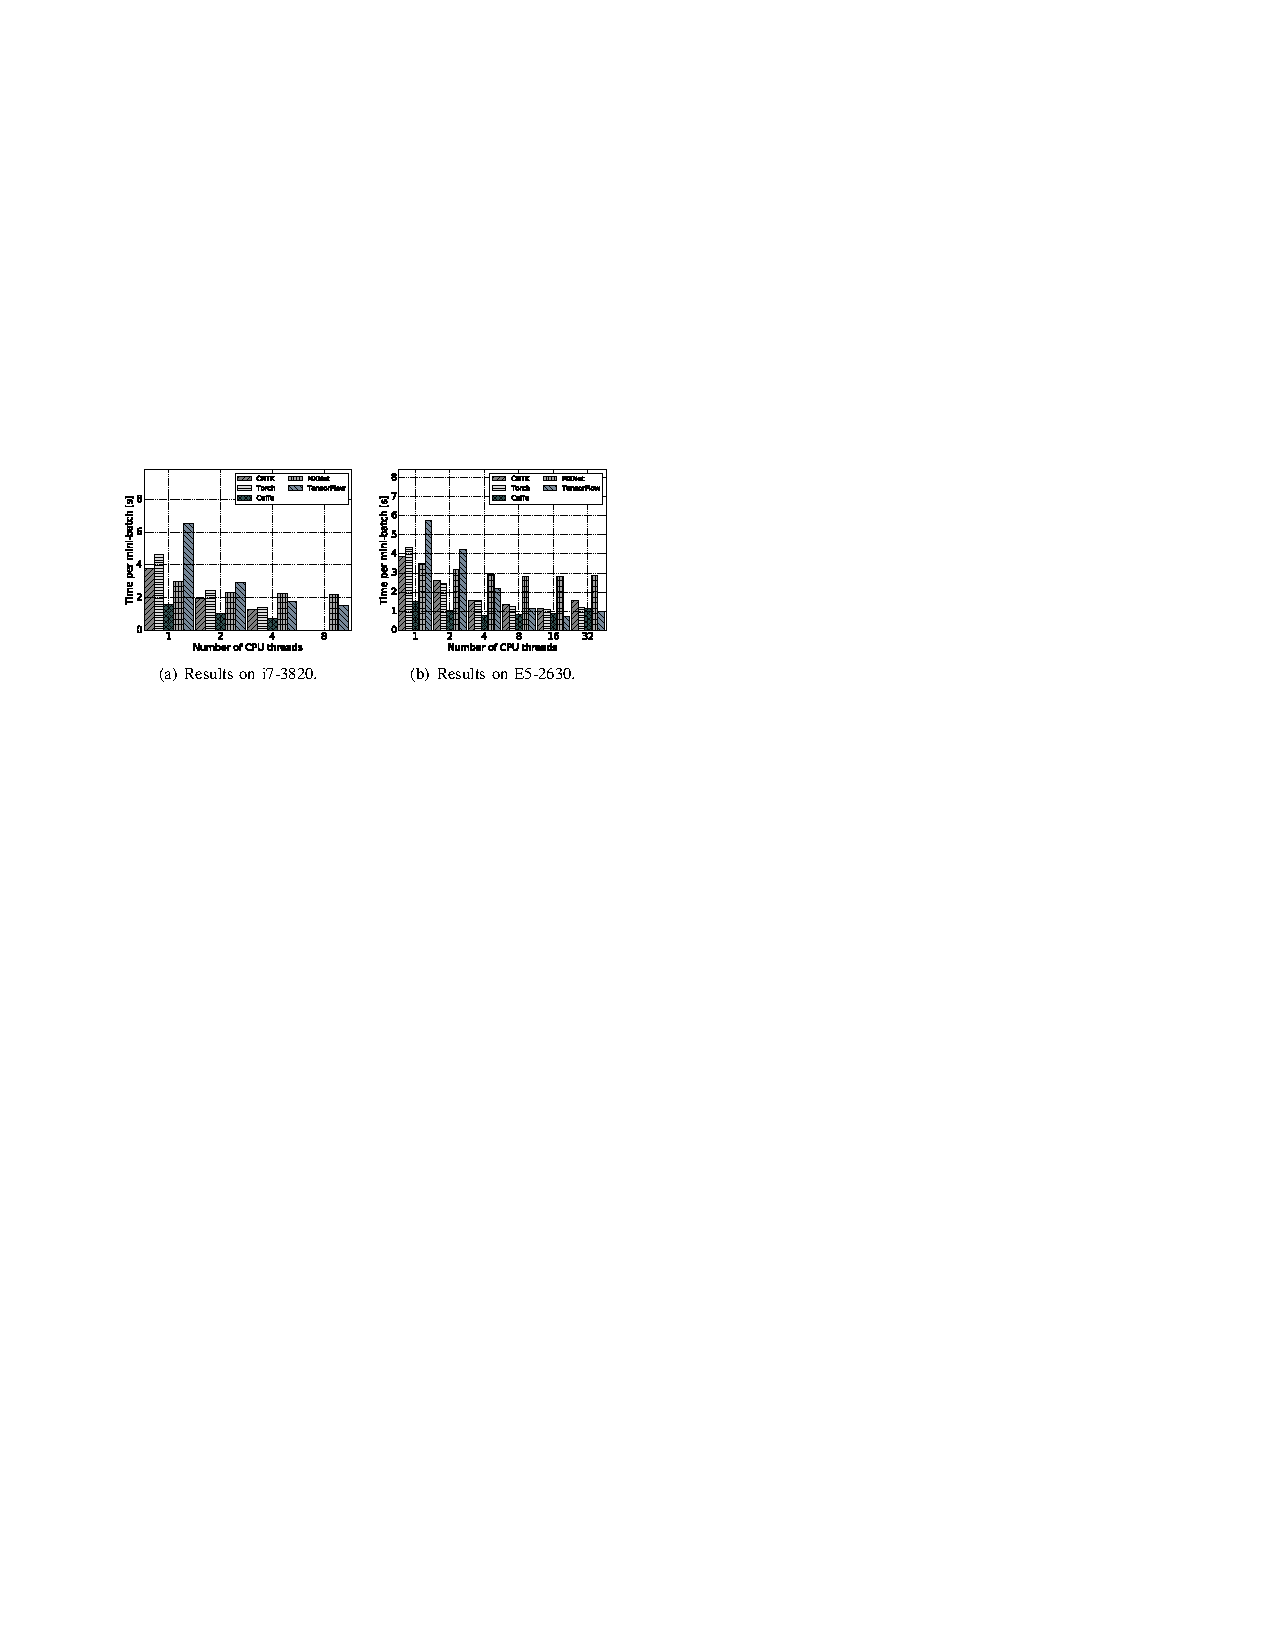
\includegraphics[width=\linewidth]{figures/AlexNet-S1.pdf} 
		\caption{AlexNet-S performance on CPU platform with a mini-batch size of 16}
	\end{figure}
	
\vskip -10pt
\begin{mdframed}[style=mystyle1]
\begin{itemize}
\item Caffe has best CNN performance as promised
\item MXNet does not scale well for this test
\end{itemize}
\end{mdframed}
	
\end{frame}

%%%

\begin{frame}
	\MyLogo
	\frametitle{CPU Scalability: CNN Real}  
	\begin{figure}[htbp] 
		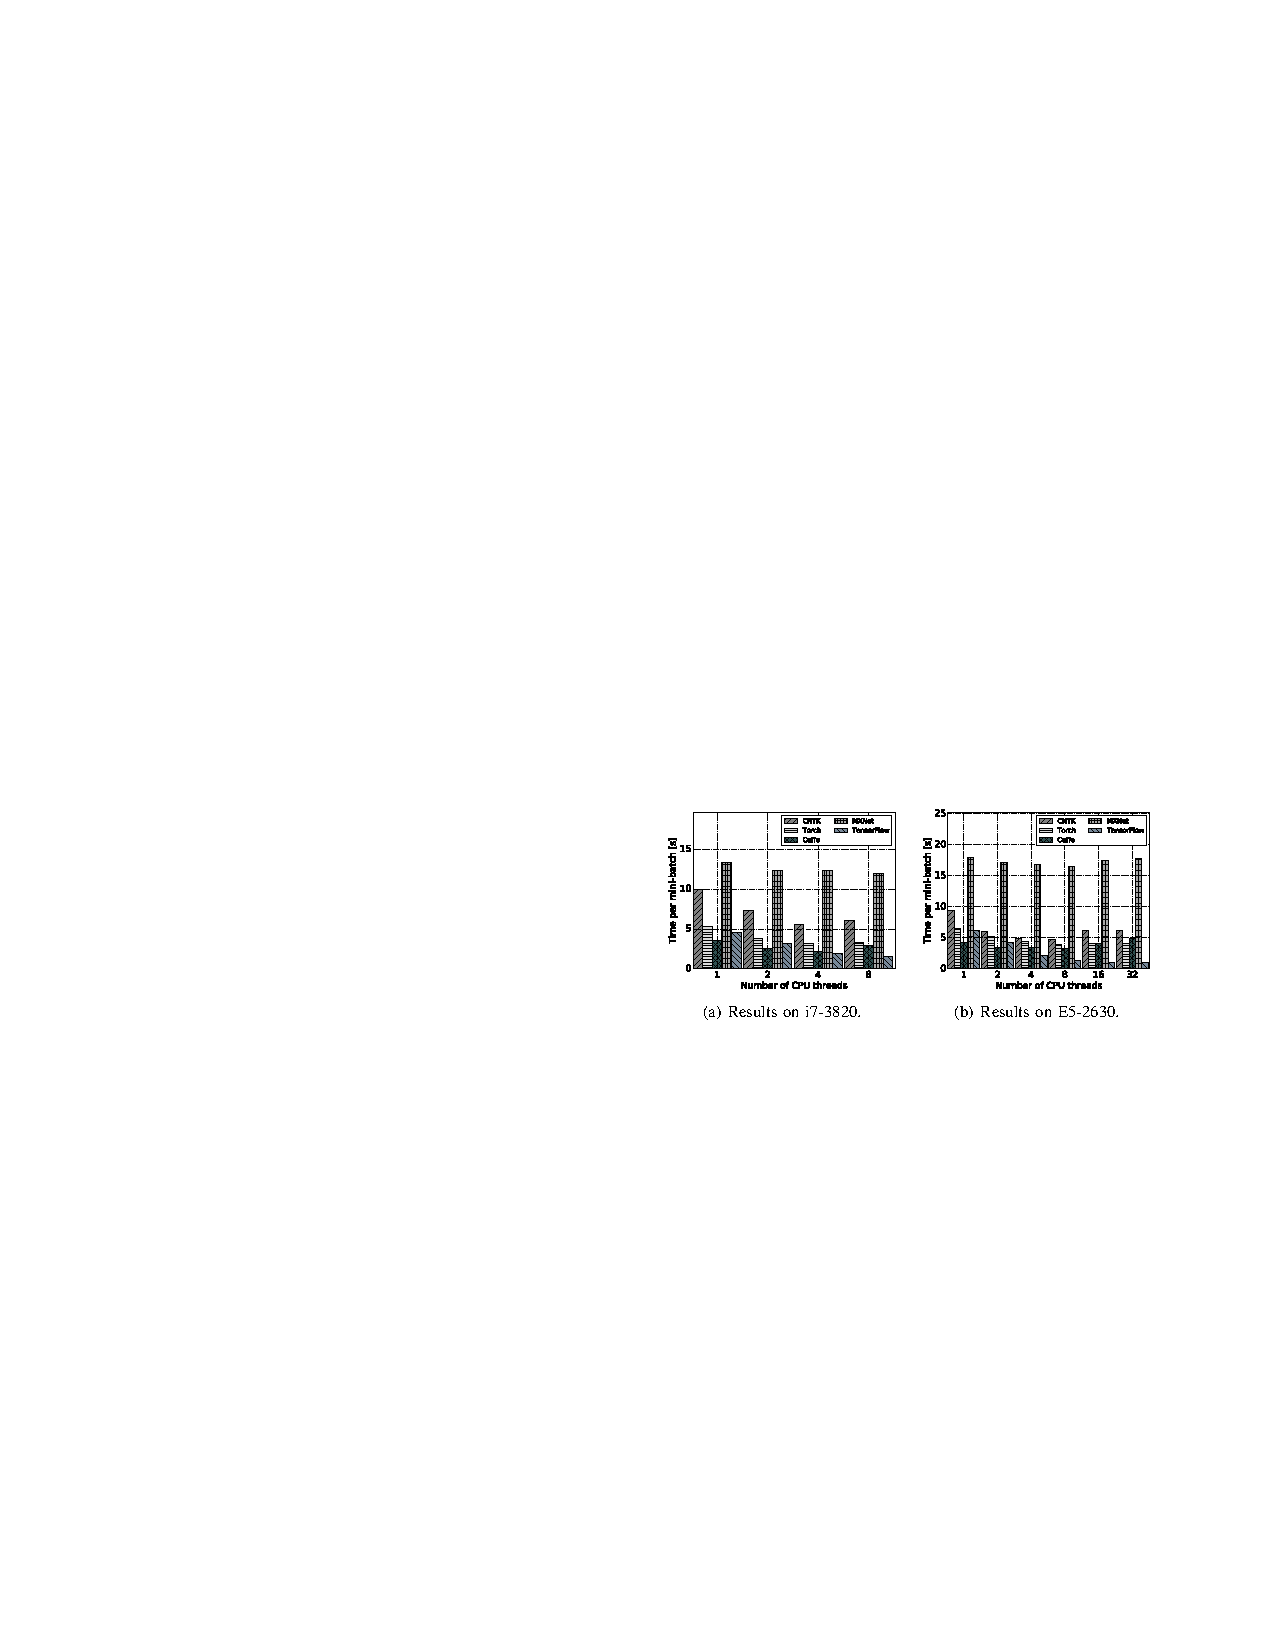
\includegraphics[width=\linewidth]{figures/AlexNet-R1.pdf} 
		\caption{AlexNet-R performance on CPU platform with a mini-batch size of 1024}
	\end{figure}
	
\vskip -10pt
\begin{mdframed}[style=mystyle1]
\begin{itemize}
\item Good scalability of TensorFlow kicks in 
\item Caffe does not scale well on multicore CPUs
\end{itemize}
\end{mdframed}

\end{frame}

%%%

\begin{frame}
	\MyLogo
	\frametitle{CPU Scalability: RNN LSTM}  
\vskip -5pt
	\begin{figure}[htbp] 
		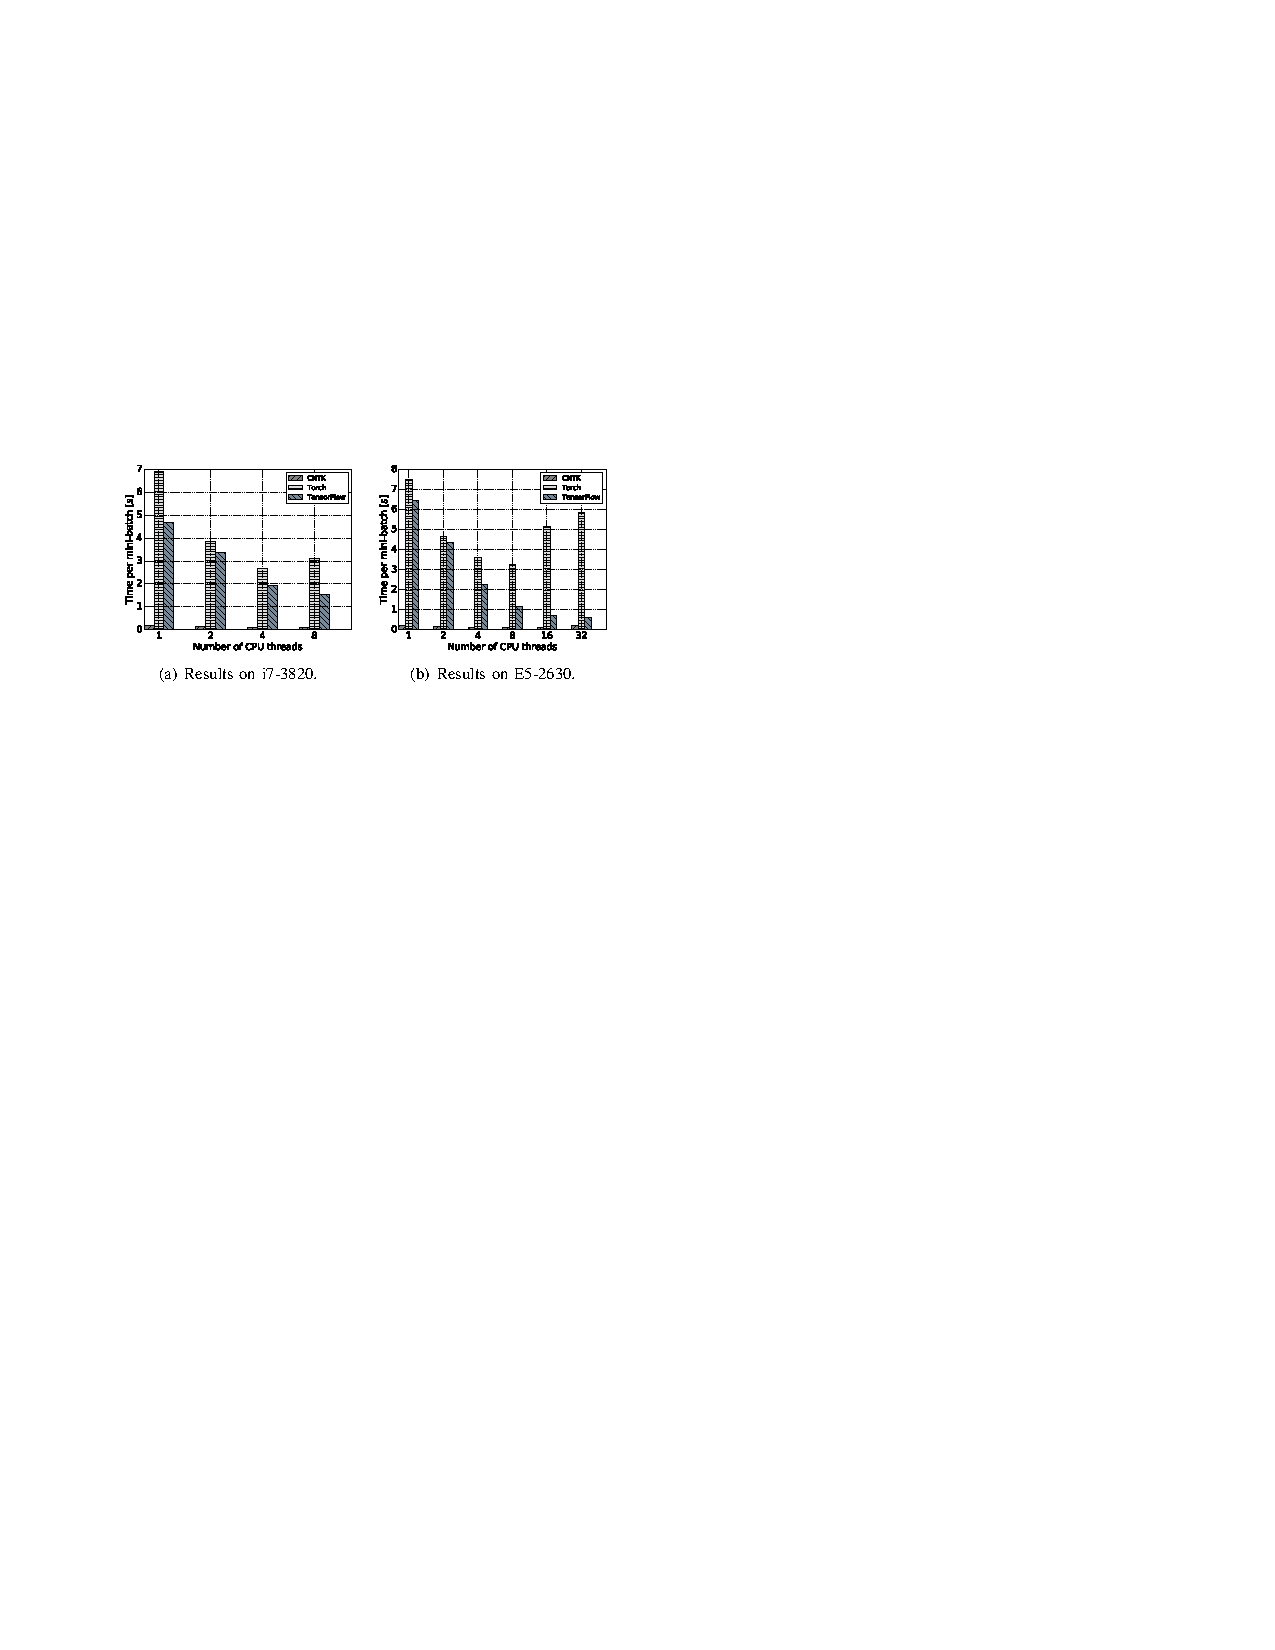
\includegraphics[width=\linewidth]{figures/LSTM1.pdf} 
		\caption{LSTM performance on CPU platform with a mini-batch size of 256}
	\end{figure}
	
\vskip -12pt
\begin{mdframed}[style=mystyle1]
\begin{itemize}
\item Pay more attention to CNTK in the future
\item Caffe/MXNet does not support LSTM on CPUs
\end{itemize}
\end{mdframed}

\end{frame}

%%%
\subsection{GPU tests}
%%%

\begin{frame}
	\MyLogo
	\frametitle{GPU Scalability: FCN Synthetic}

	\begin{figure}[htbp] 
		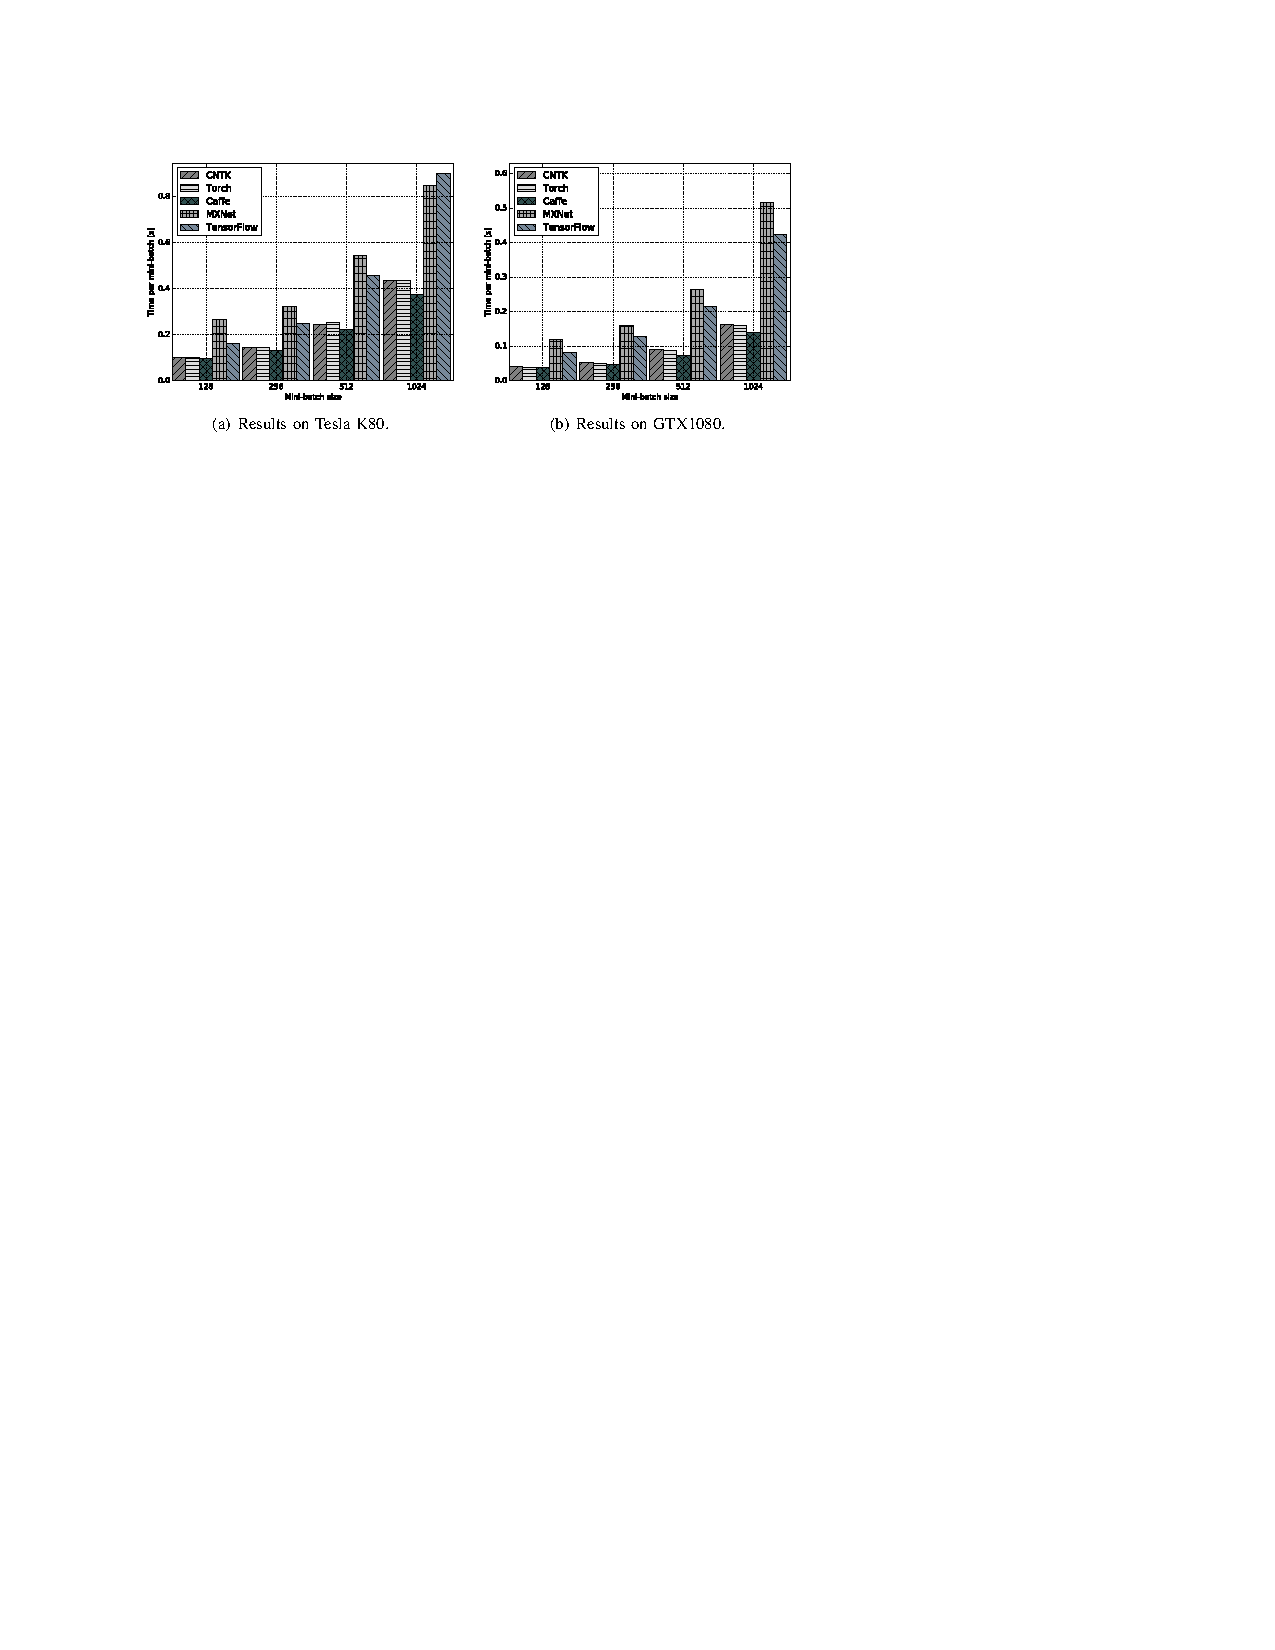
\includegraphics[width=\linewidth]{figures/FCN-S2.pdf} 
		\caption{The performance comparison of FCN-S on GPU platforms}
	\end{figure}

\vskip -10pt
\begin{mdframed}[style=mystyle1]
\begin{itemize}
\item CNTK/Torch/Caffe out-perform the others
\end{itemize}
\end{mdframed}

\end{frame}

%%%

\begin{frame}
	\MyLogo
	\frametitle{GPU Speed: FCN Real}
	
	\begin{figure}[htbp] 
		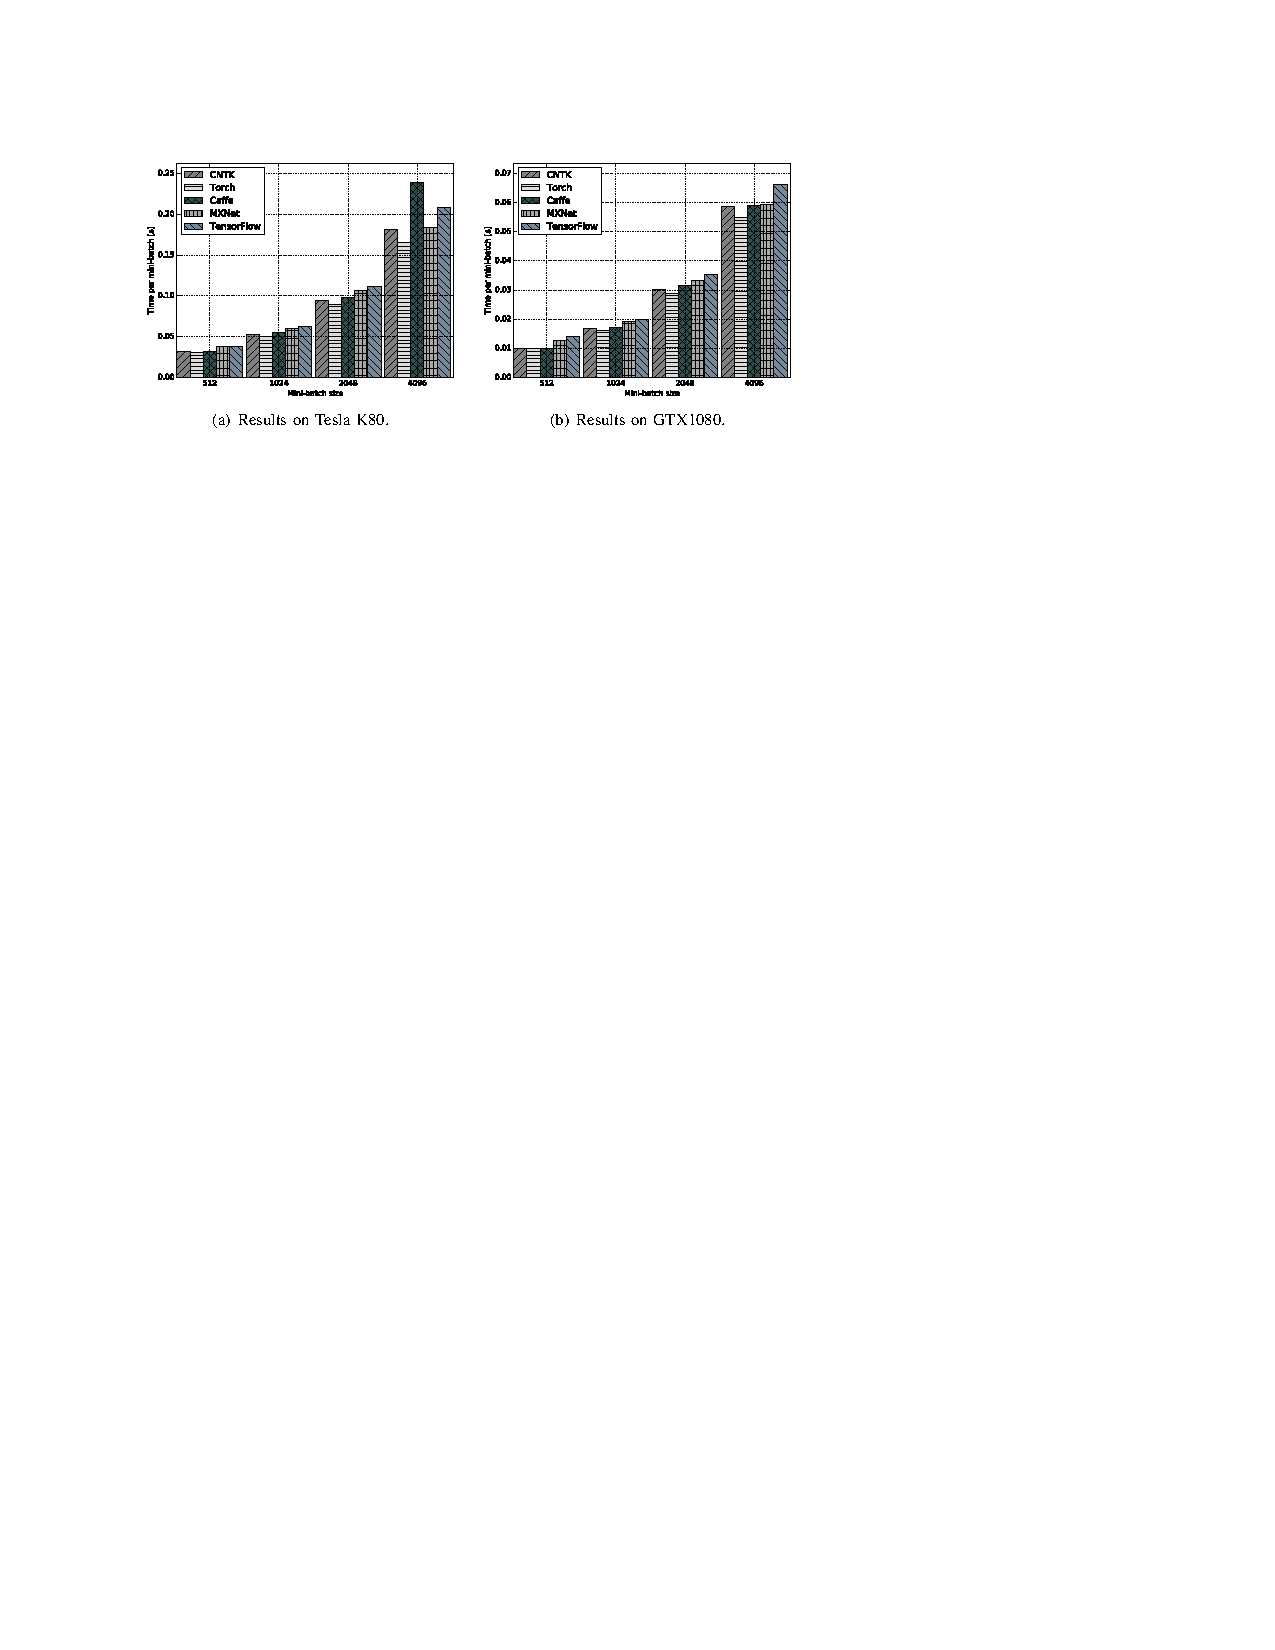
\includegraphics[width=\linewidth]{figures/FCN-R2.pdf} 
		\caption{The performance comparison of FCN-R on GPU platforms}
	\end{figure}

\vskip -10pt
\begin{mdframed}[style=mystyle1]
\begin{itemize}
\item All packages have similar performance
\end{itemize}
\end{mdframed}

\end{frame}

%%%

\begin{frame}
	\MyLogo
	\frametitle{GPU Speed: CNN Synthetic}

	\begin{figure}[htbp] 
		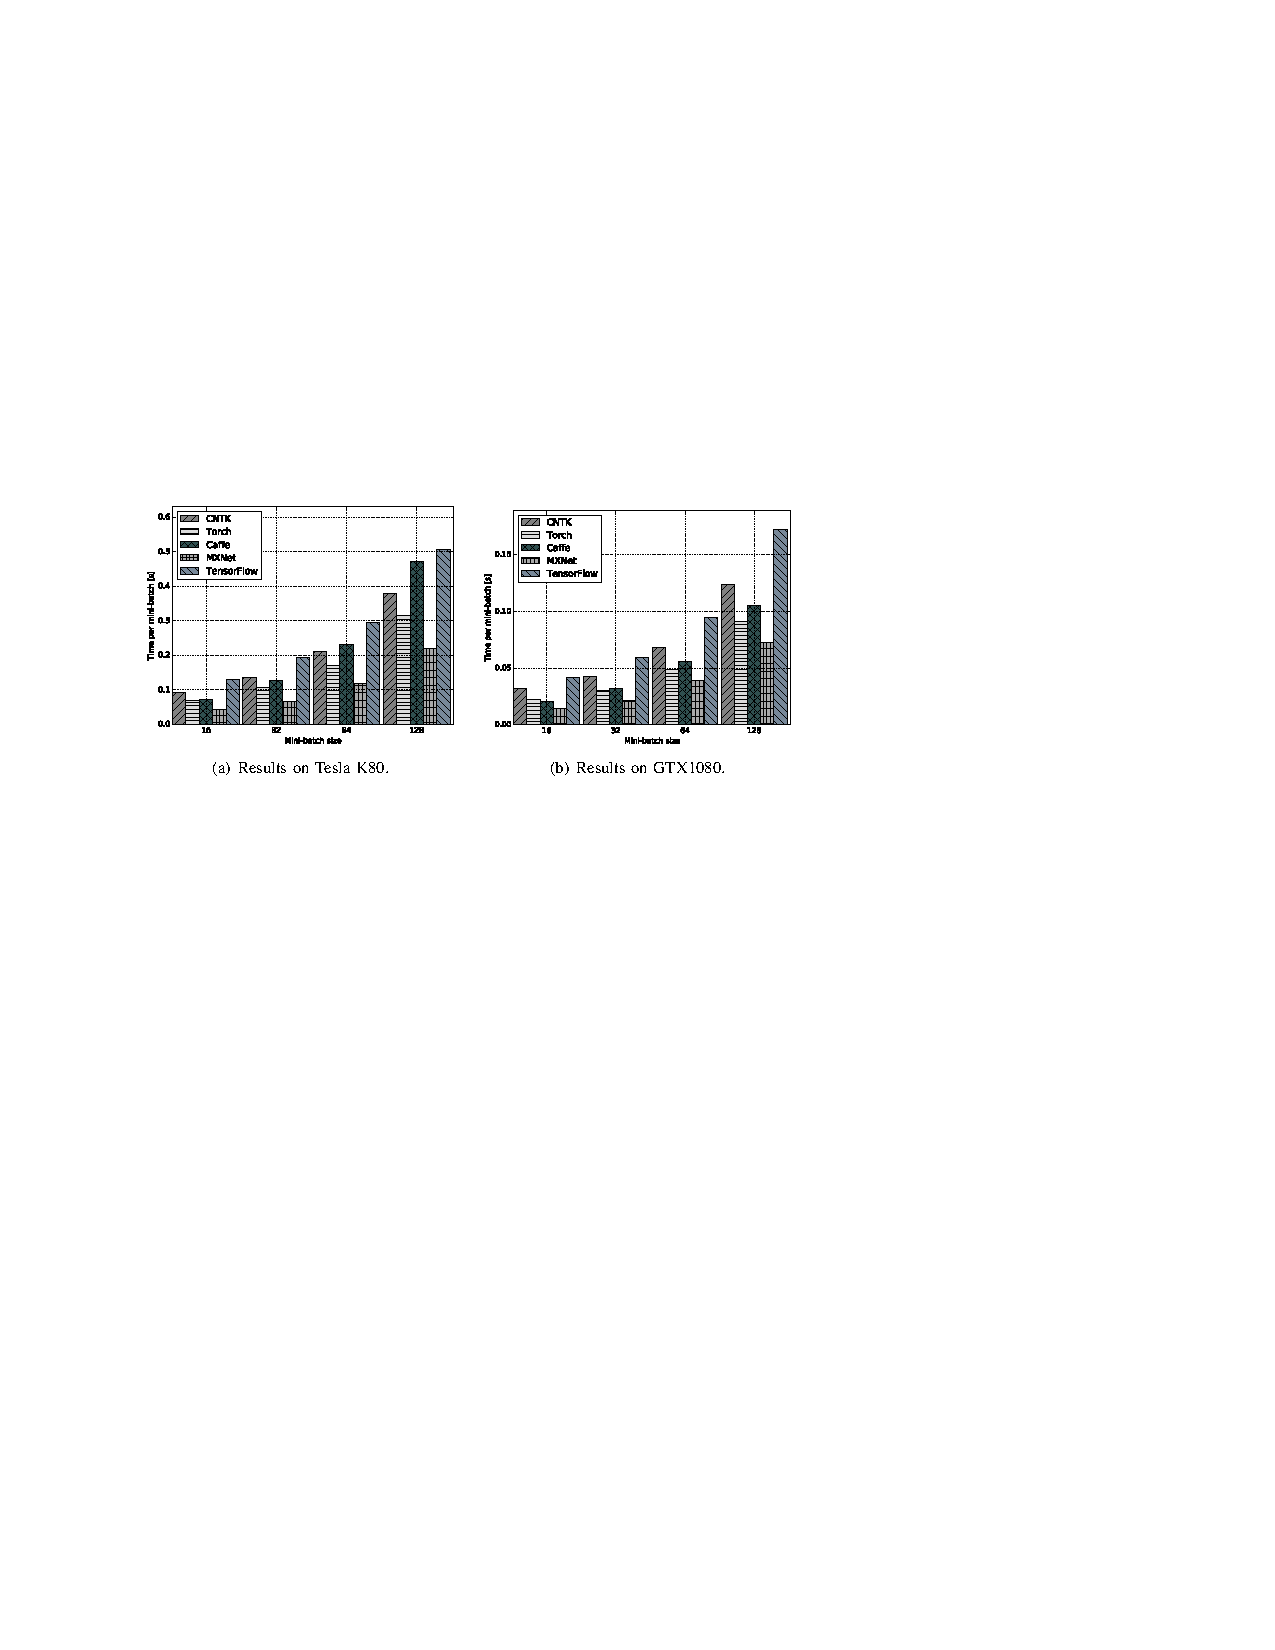
\includegraphics[width=\linewidth]{figures/AlexNet-S2.pdf} 
		\caption{The performance comparison of AlexNet-S on GPU platforms}
	\end{figure}

\vskip -10pt
\begin{mdframed}[style=mystyle1]
\begin{itemize}
\item MXNet out-perform the others for CNN on GPUs
\end{itemize}
\end{mdframed}

\end{frame}

%%%

\begin{frame}
	\MyLogo
	\frametitle{GPU Speed: CNN Real}

	\begin{figure}[htbp] 
		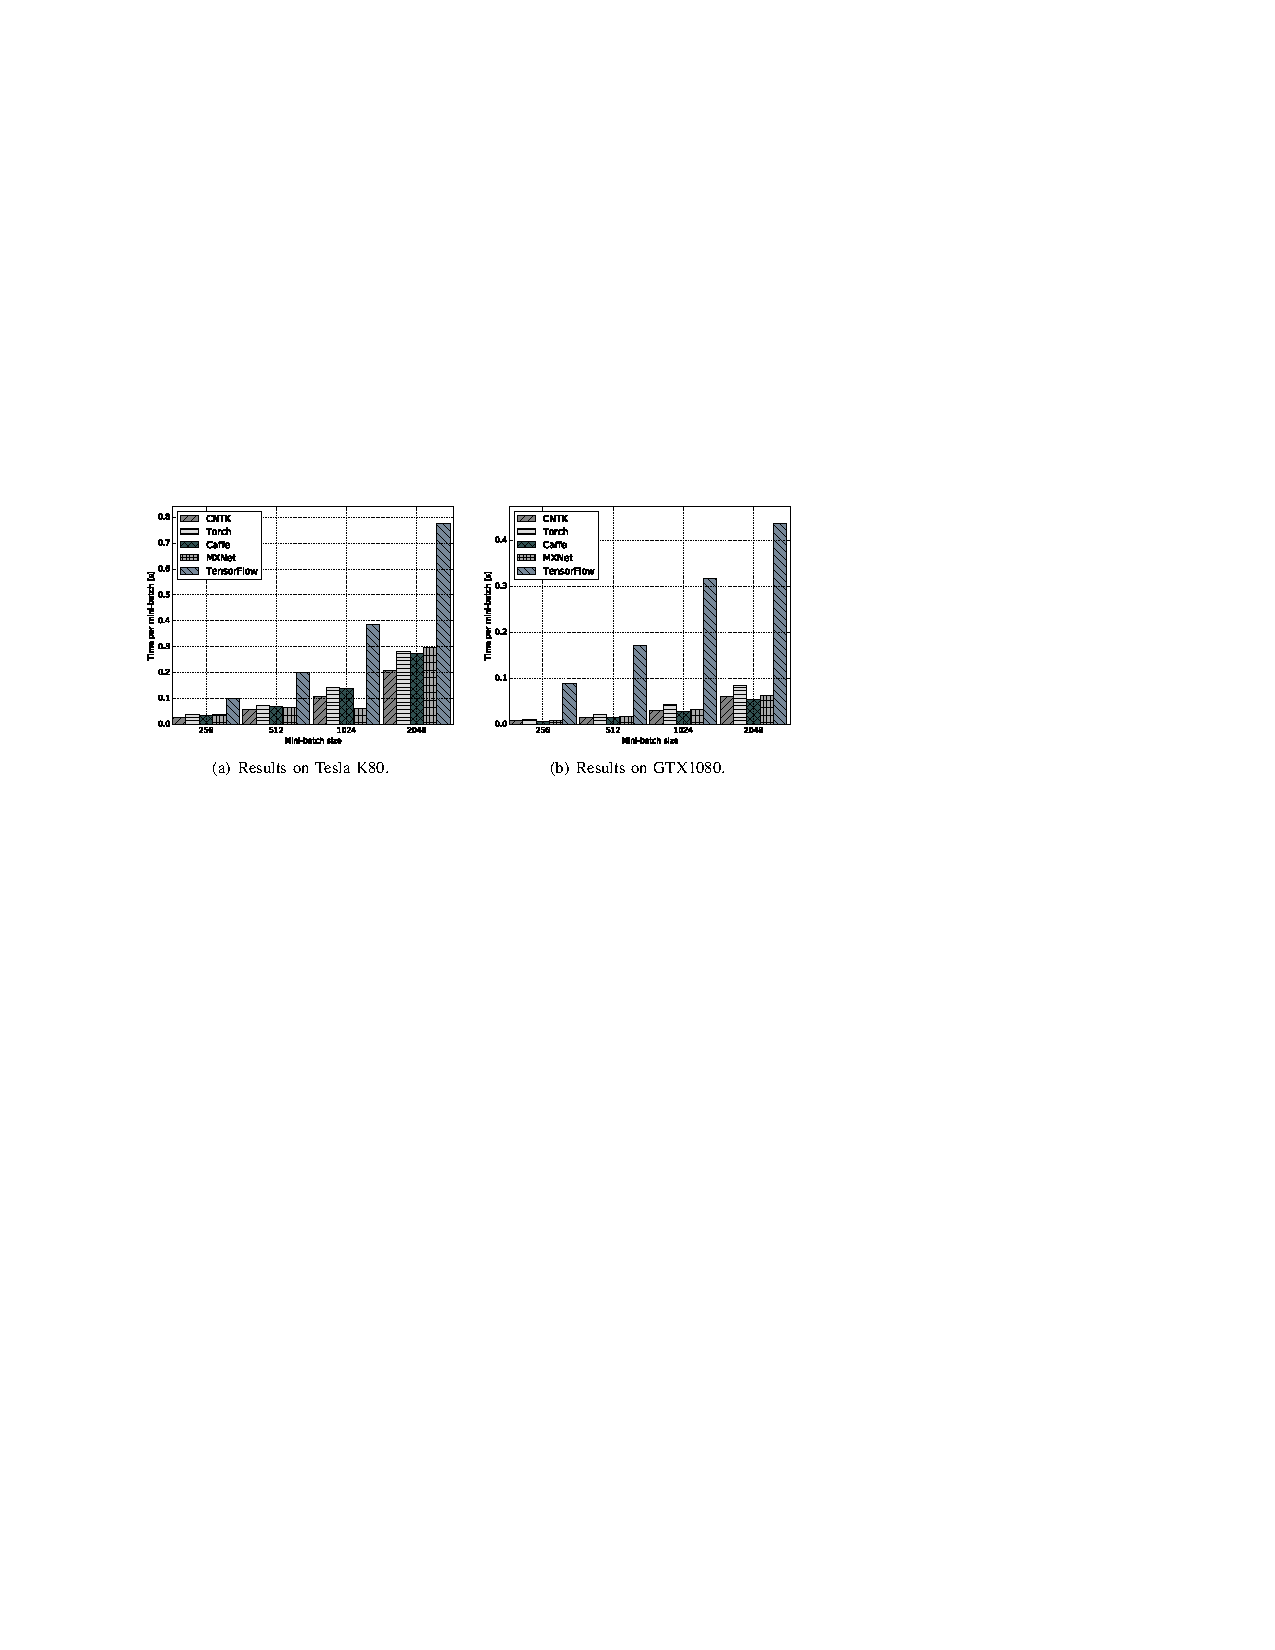
\includegraphics[width=\linewidth]{figures/AlexNet-R2.pdf} 
		\caption{The performance comparison of AlexNet-R on GPU platforms}
	\end{figure}

\vskip -10pt
\begin{mdframed}[style=mystyle1]
\begin{itemize}
\item TensorFlow does not have good GPU performance in general
\end{itemize}
\end{mdframed}

\end{frame}

%%%

\begin{frame}
	\MyLogo
	\frametitle{GPU Speed: RNN LSTM}
	
	\begin{figure}[htbp] 
		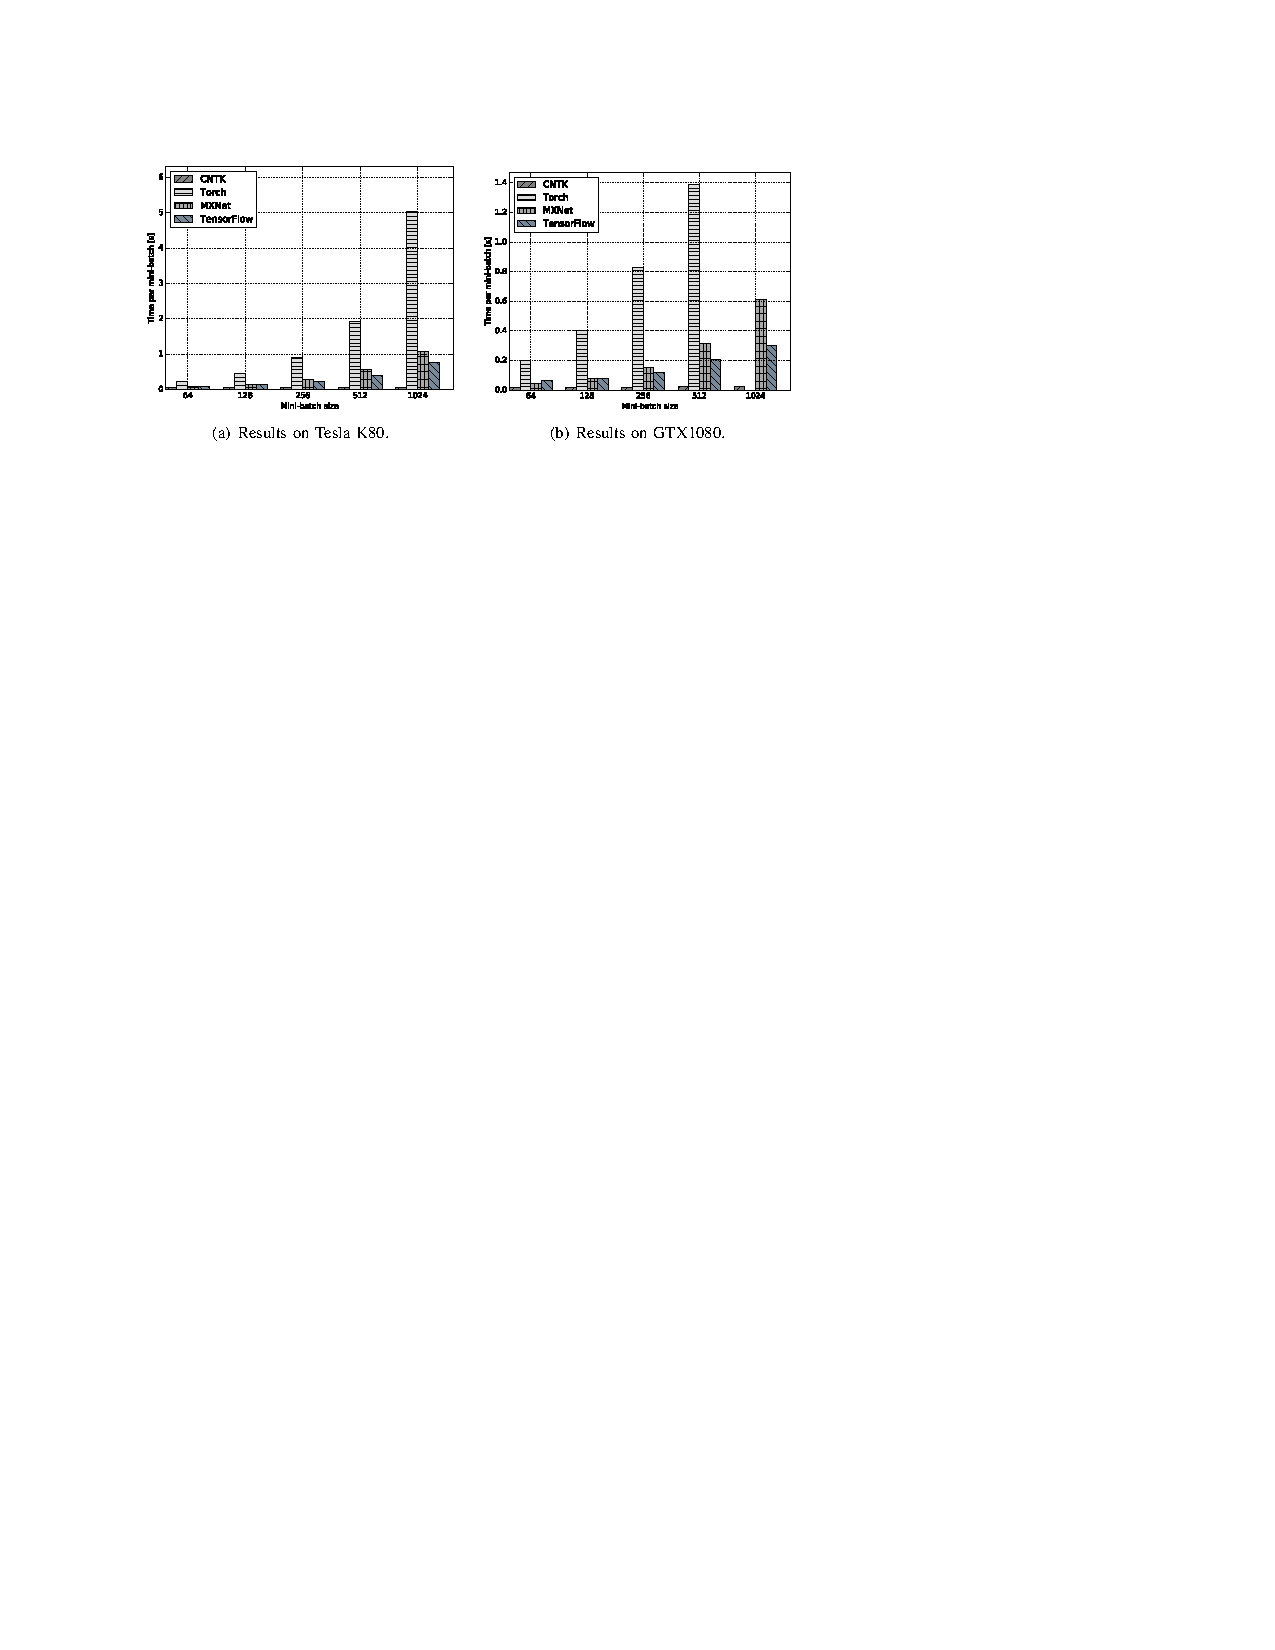
\includegraphics[width=\linewidth]{figures/LSTM2.pdf} 
		\caption{The performance comparison of LSTM on GPU platforms}
	\end{figure}

\vskip -10pt
\begin{mdframed}[style=mystyle1]
\begin{itemize}
\item CNTK has excellent RNN performance both on CPU and GPU
\end{itemize}
\end{mdframed}
	
\end{frame}


\begin{frame}
	\MyLogo
	\frametitle{Multi-GPU Scalability}
	
\vskip -10pt
\begin{figure}[!htbp]%[H]
\centering
\subfloat[Subfigure 1 list of figures text][FCN-R]{
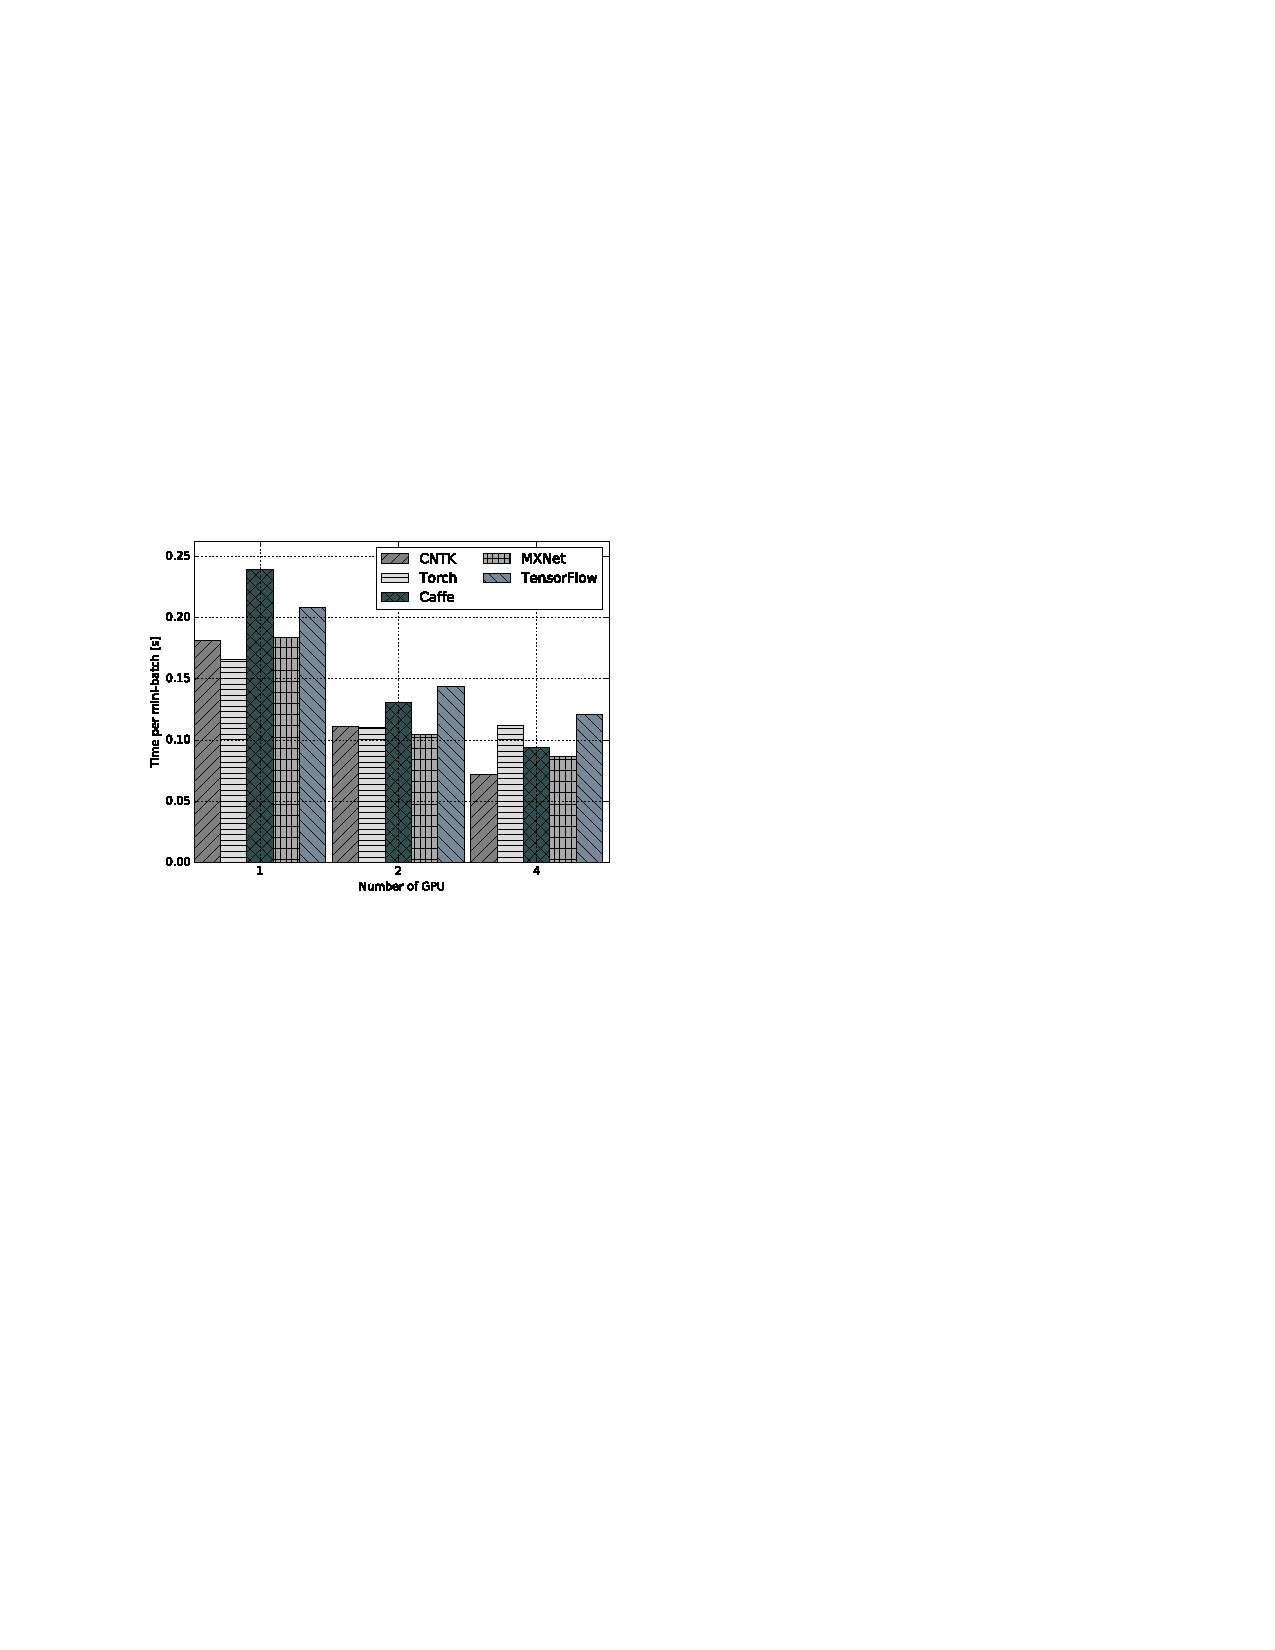
\includegraphics[width=0.48\textwidth]{figures/16a.pdf}
}
\subfloat[Subfigure 2 list of figures text][CNN-R]{
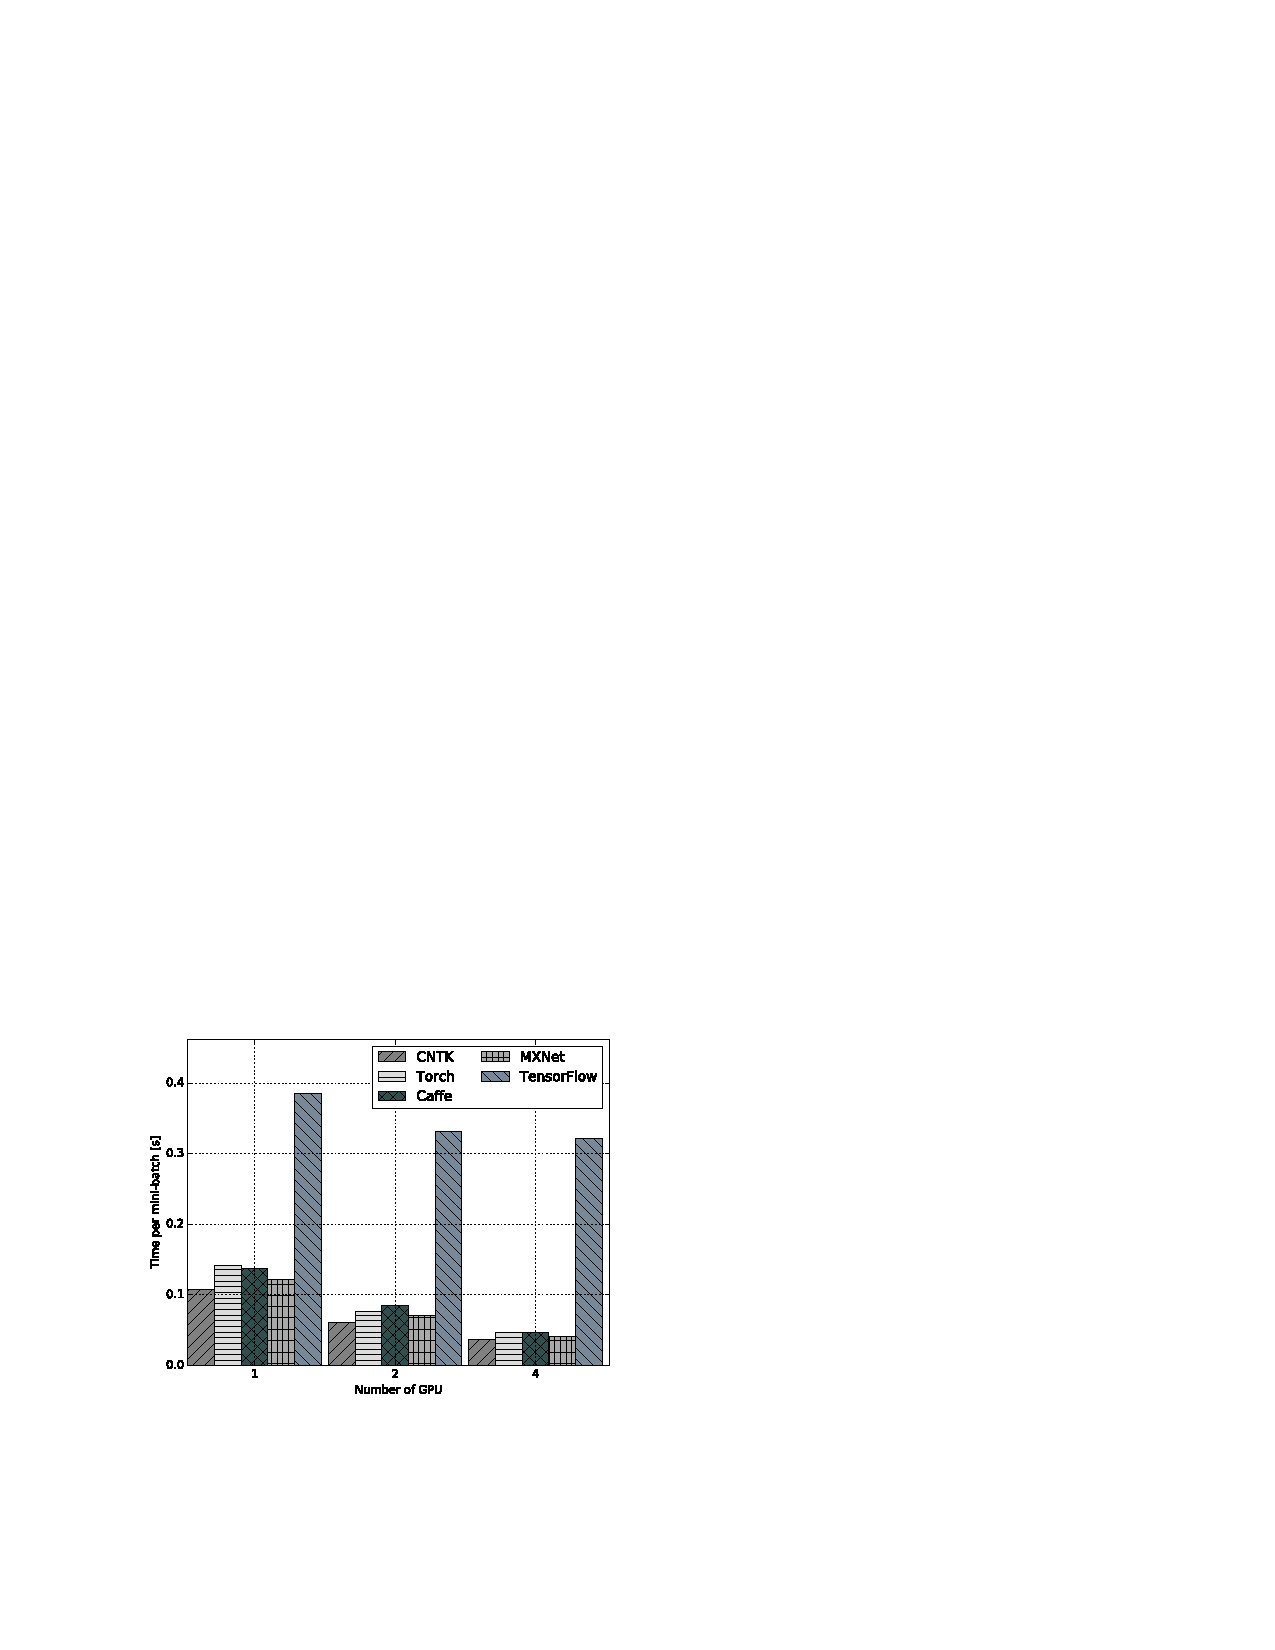
\includegraphics[width=0.48\textwidth]{figures/17a.pdf}
}
\caption{The scalability on a multi-GPU platform (2 $\times$ K80)}
\end{figure}

\vskip -10pt
\begin{mdframed}[style=mystyle1]
\begin{itemize}
\item Multi-GPU can greatly boost the training process of network
\item MXNet shows overwhelming advantage over the others
\item TensorFlow does not scale well on multi-GPU platform
\end{itemize}
\end{mdframed}
\end{frame}
